\documentclass[12pt]{article}
\usepackage[utf8]{inputenc}
\usepackage[T1]{fontenc}
\usepackage{graphicx}
\usepackage{xcolor}
\usepackage{hyperref}
\usepackage{wrapfig}
\usepackage{listings}
\usepackage{booktabs}
\usepackage{colortbl}
\usepackage{amsmath}
\usepackage{xparse}

\definecolor{eclipseStrings}{RGB}{42,0.0,255}
\definecolor{eclipseKeywords}{RGB}{127,0,85}
\definecolor{jsonbackground}{RGB}{217, 237, 250}
\colorlet{numb}{magenta!60!black}

\definecolor{dkgreen}{rgb}{0,0.6,0}
\definecolor{gray}{rgb}{0.5,0.5,0.5}
\definecolor{mauve}{rgb}{0.58,0,0.82}

\lstset{frame=tb,
language=R,
keywordstyle=\color{blue},
alsoletter={.},
otherkeywords={!=, ~, $, *, \&, \%/\%, \%*\%, \%\%, <-, <<-, /},
deletekeywords={c, data, get, aggregate, summary}
}





\NewDocumentCommand{\codeword}{v}{%
\texttt{\textcolor{blue}{#1}}%
}


\lstdefinelanguage{json}{
    basicstyle=\normalfont\ttfamily,
    commentstyle=\color{eclipseStrings}, % style of comment
    stringstyle=\color{eclipseKeywords}, % style of strings
    numberstyle=\scriptsize,
    stepnumber=1,
    numbersep=8pt,
    showstringspaces=false,
    breaklines=true,
    backgroundcolor=\color{jsonbackground}, %only if you like
    string=[s]{"}{"},
    comment=[l]{:\ "},
    morecomment=[l]{:"},
    literate=
        *{0}{{{\color{numb}0}}}{1}
         {1}{{{\color{numb}1}}}{1}
         {2}{{{\color{numb}2}}}{1}
         {3}{{{\color{numb}3}}}{1}
         {4}{{{\color{numb}4}}}{1}
         {5}{{{\color{numb}5}}}{1}
         {6}{{{\color{numb}6}}}{1}
         {7}{{{\color{numb}7}}}{1}
         {8}{{{\color{numb}8}}}{1}
         {9}{{{\color{numb}9}}}{1}
}

%%novalidate

\usepackage{tikz}
\usepackage{calc}
\usepackage{booktabs}
%\usepackage{hyperref}

% colors
\definecolor{color1}{RGB}{10,23,55}
%\definecolor{color1}{HTML}{8C260F}
\definecolor{color2}{RGB}{10,23,55}
\definecolor{statsorange}{RGB}{237,105,36}


% fonts
\usepackage{fontspec}
\defaultfontfeatures{Mapping=tex-text}
\setmainfont
[BoldFont=Lato-Bold.ttf,
ItalicFont=Lato-Italic.ttf,
BoldItalicFont=Lato-BoldItalic.ttf]
{Lato-Regular.ttf}
\newfontfamily\headingfont[ItalicFont=Lato-BlackItalic.ttf]{Lato-Black.ttf}
%%%

\usepackage{geometry}
\geometry{a4paper,
hmargin=20mm,vmargin=30mm,
head=0ex,foot=3ex}

\linespread{1.3}

\usepackage[hang]{caption}

\captionsetup{labelfont={bf,color=color2},textfont={normalsize,color=color2},figurename=FIGURE,tablename=TABLE}

%%% fancy sections
\usepackage{titlesec}
%\titleformat{\chapter}{\headingfont\LARGE\bfseries\scshape\color{color1}}{\thechapter}{1em}{}[\titlerule]
\titleformat{\section}{\color{color1}\headingfont\Large\bfseries\uppercase}{\thesection}{1em}{}
\titleformat{\subsection}{\color{color1}\headingfont\large\bfseries\uppercase}{\thesubsection}{1em}{}
\titleformat{\subsubsection}{\color{color1}\headingfont\bfseries\uppercase}{\thesubsubsection}{1em}{}
%%%

% head and foot
\usepackage{fancyhdr}
\pagestyle{fancy}
\lhead{}
\chead{}
\makeatletter
\rhead{\color{color2}\@date}
\makeatother
\newlength{\myheight}
\lfoot{
\settoheight{\myheight}{\thepage}

\includegraphics[height=10.5ex]{icon-900px}
}
\cfoot{\color{color2}}
\rfoot{\raisebox{5ex-0.5\myheight}{\color{color2}Generic data portals | \bf{Page \thepage}}}
\renewcommand\headrulewidth{0pt}
\renewcommand\footrulewidth{0pt}


\newcommand{\placetextbox}[3]{% \placetextbox{<horizontal pos>}{<vertical pos>}{<stuff>}
  \setbox0=\hbox{#3}% Put <stuff> in a box
  \AddToShipoutPictureFG*{% Add <stuff> to current page foreground
    \put(\LenToUnit{#1\paperwidth},\LenToUnit{#2\paperheight}){\vtop{{\null}\makebox[0pt][c]{#3}}}%
  }%
}%

%%% picture on cover page
\usepackage{eso-pic}
\newcommand\BackgroundPic{%
\put(0,0){%
\parbox[b][\paperheight]{\paperwidth}{%
\vfill
\centering

\includegraphics[width=\paperwidth,height=\paperheight,%
keepaspectratio]{cover}%
\vfill
}}}
%%%
% custom titlepage
\makeatletter
\renewcommand{\maketitle}{
\thispagestyle{empty}
\AddToShipoutPicture*{\BackgroundPic}
\ClearShipoutPicture
%
\vfill
\begin{tabular}[c]{@{}p{0.7\textwidth}@{}}
      
\end{tabular}
\placetextbox{0.28}{0.85}{
{\color{color1}\headingfont\Huge\@title\\[2em]}}
\placetextbox{0.43}{0.8}{{\color{color1}\headingfont\Huge\@author\\[1em]}\color{statsorange}{\headingfont\Huge .}}
%
\clearpage
}
\makeatother
%%%


%%% fancy boxes
\usepackage{tcolorbox}
\usepackage{wrapfig}
\def\fullboxbegin{
\bigskip
\begin{tcolorbox}[colback=color1,colframe=color1,coltext=white,arc=0mm,boxrule=0pt]
}
\def\fullboxend{\end{tcolorbox}\medskip}
%
\def\leftboxbegin{
\begin{wrapfigure}{l}{0.5\textwidth}
\begin{tcolorbox}[colback=color1,colframe=color1,coltext=white,arc=0mm,boxrule=0pt]
}
\def\leftboxend{
\end{tcolorbox}
\end{wrapfigure}
}
%
\def\rightboxbegin{
\begin{wrapfigure}{r}{0.5\textwidth}
\begin{tcolorbox}[colback=color1,colframe=color1,coltext=white,arc=0mm,boxrule=0pt]
}
\def\rightboxend{
\end{tcolorbox}
\end{wrapfigure}
}
%
\newcounter{frames}
\def\frameboxbegin#1{
\bigskip
\refstepcounter{frames}
\begin{tcolorbox}[colback=white,colframe=color1,arc=0mm,title={\MakeUppercase{\textbf{Frame \arabic{frames}}: #1}}]
}
\def\frameboxend{
\end{tcolorbox}
}
%%%

\newcommand\statssection[1]{%
  \section*{\MakeUppercase{#1}}
  \raisebox{1.5em}[0pt][0pt]{\textcolor{statsorange}{\rule{0.2\textwidth}{6pt}}}
}


%%%%%%%%%%%%%%%
% Title Page
\title{Generic data portals}
\author{Documentation and process outline}
\date{\today}
%%%%%%%%%%%%%%%

\begin{document}
\maketitle

%\tableofcontents
\clearpage
\setcounter{page}{1}


{\center\vspace{1cm} \ \ }

{\center\textbf{For feedback or queries contact  \href{mailto:james.mckay@stats.govt.nz}{james.mckay@stats.govt.nz} }.}

\vspace{1cm}

\statssection{Introduction}

The publication of a large number of unique data sets in a user friendly visualisation can present a challenging problem.  This is often solved through the production of a specialised \textit{dashboard} for the particular data set and audience.  However, these solutions can become complicated, expensive to maintain and can be difficult to recycle for new data.




\vspace{0.5cm}

\begin{figure}[h]
\centering
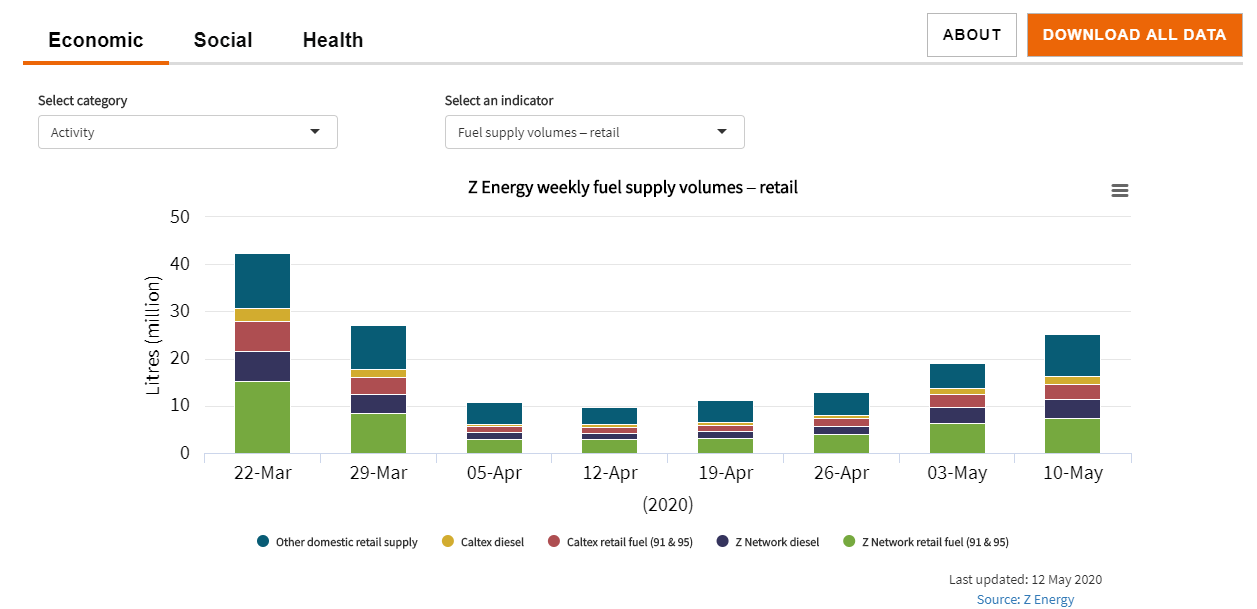
\includegraphics[width=\textwidth]{figures/data_portal.png}
 	\caption{The Stats NZ COVID-19 Data Portal.}\label{fig:covid_19_portal}
\end{figure}
This documentation describes the data management princinples and software used to produce the COVID-19 data portal shown in Figure \ref{fig:covid_19_portal}.  The intended use of this documentation, and the associated code, is for the reuse of this solution for rapid production of data visualisations.

\clearpage
\statssection{The data management process}\label{sec:data}
\begin{wrapfigure}{r}{0.5\textwidth}
\centering
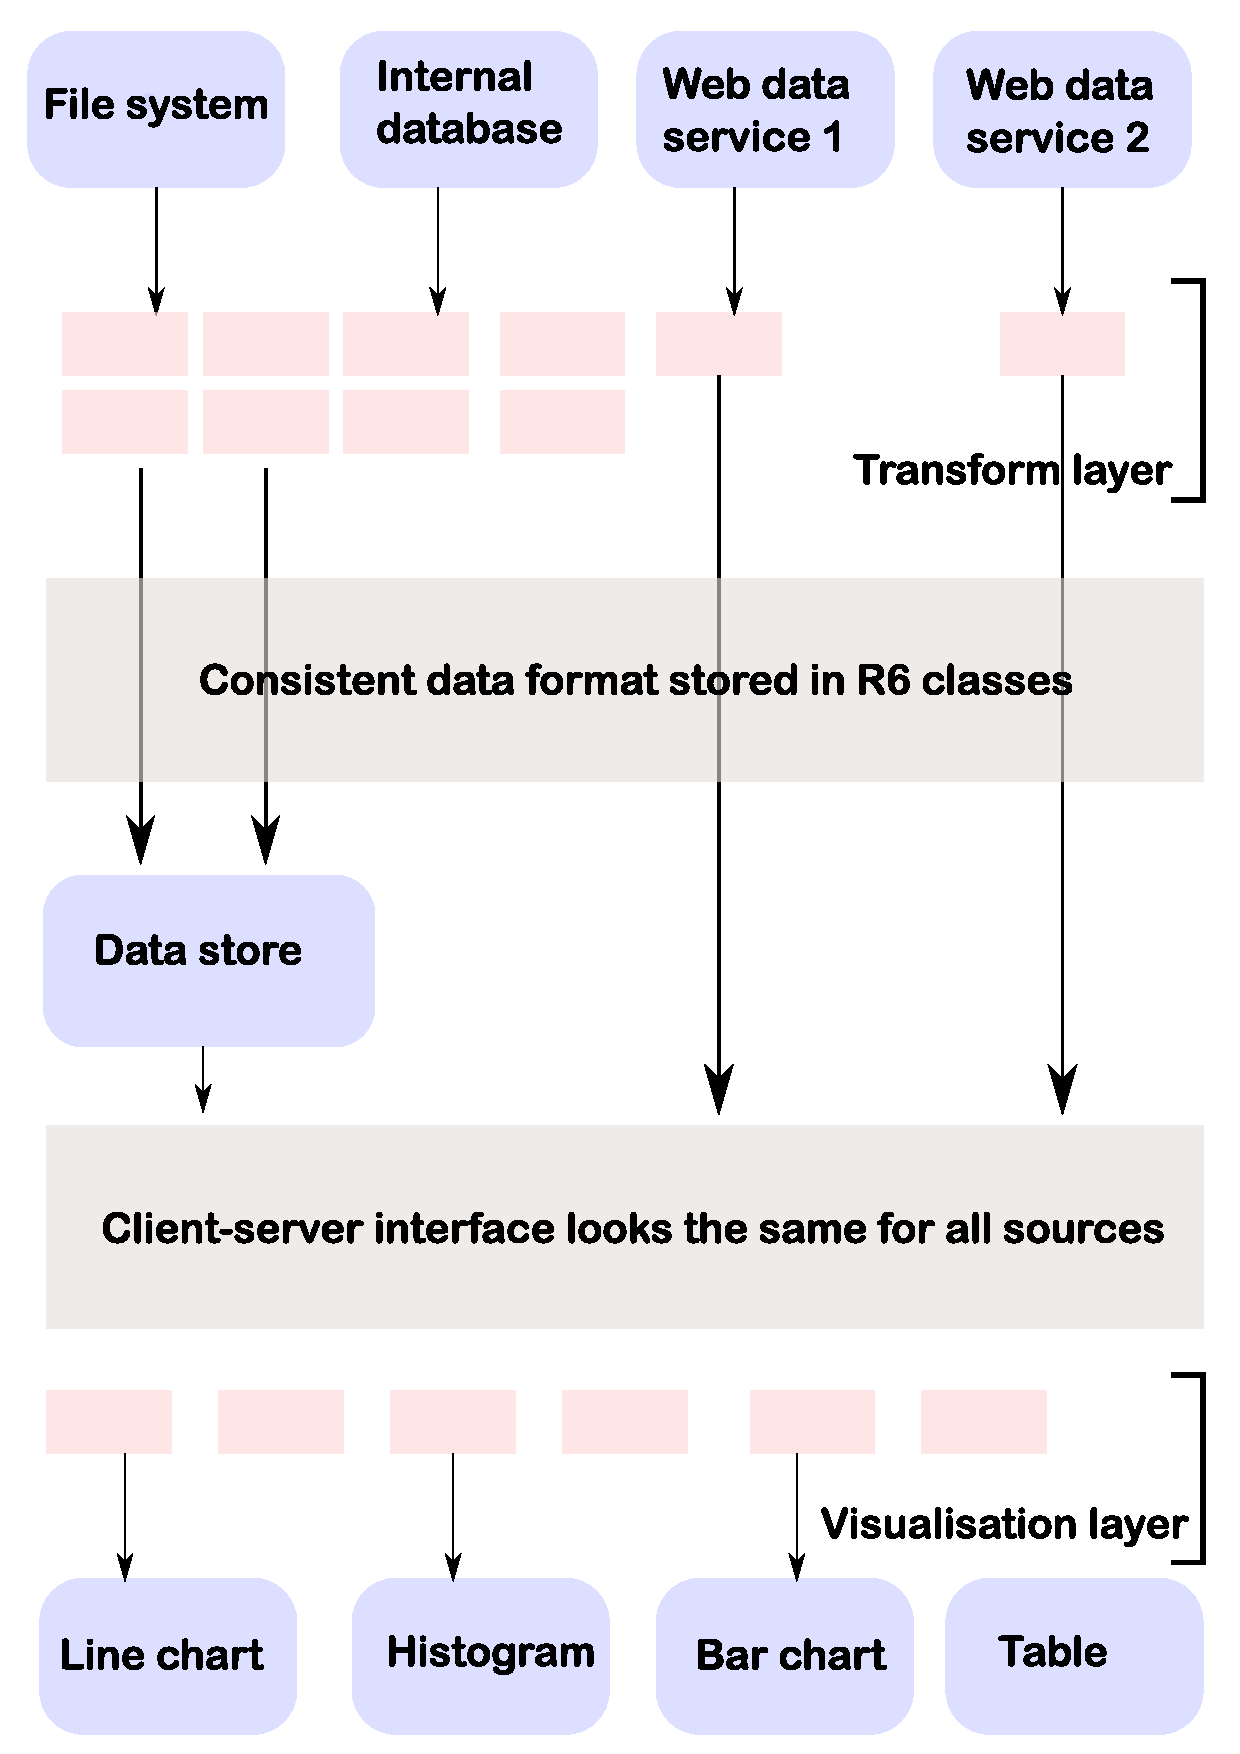
\includegraphics[width=0.5\textwidth]{figures/data_process.pdf}
 	\caption{The data process.}\label{fig:data_process}
\end{wrapfigure}
For this application to be able to scale quickly and be reused for a range of needs there must be a robust and flexible data management process.  In Figure \ref{fig:data_process} we show the process map for the various types of data sources and how these flow through the system.

In Figure \ref{fig:data_process} we show four possible sources of data at the top.  These represent the first steady-state.  The original raw data is read in using either one of the predefined functions, or by writting a custom function if a new source is required (such as a new web service).  For a file this is as simple as pointing to the correct directory, so there is little abstraction required -- but web services or database calls may require specific functions.  This raw data is then passed into the transformation layer.  This layer may contain many custom \textit{load functions} designed to transform raw data into a consistent format.  The output of these load functions must be a type defined in \codeword{R/data_types.R}.  If a suitable structure is not available then one can be defined in that file.

Internal data is then passed into the \textit{data store}.  This is simple a list containing all the data sets saved into a file on the harddrive.  This file is then deployed with the application.

Finally all data is accessible through the client-service interface.  From the perspective of the client this layer is called in the same way with the same behaviour regardless of the data source, returning one of the expected data types.  This data is then passed through the visualisation layer, where custom plot functions may be defined for alternative visualisations of data.

\newpage
\clearpage
\statssection{Code documentation}

The rest of this document outlines how to work with the Shiny application to produce a data portal for a new use case.  The best place to start to get familiar with the code is by running the example.  To run the example do the following steps.
\begin{enumerate}
\item Copy the file \codeword{config/example_config.yaml} into a new file called \codeword{config/config.yaml} (this file is not to be kept under version control as it's specific to each deployment).
\item Run the script \codeword{scripts/run_load_process.R}.
\item Run the command \codeword{shiny::runApp(".")} to start the application.
\end{enumerate}

This will use the indicator and data definitions defined in \codeword{config/example_indicators.json} and \codeword{config/example_data_definitions.json} to create a visualisation.


\subsection*{Defining indicators}

Indicators are defined in a JSON format configuration file.  For each indicator this defines all properties such as the titles, labels, the source of the data and any additional parameters required to request that data.

All visualisations in the application must have a unique key, which is a concatenation of
\begin{itemize}
\item The \codeword{class}
\item The \codeword{type}
\item The \codeword{indicator_name}
\item The \codeword{name} parameter of the group
\end{itemize}
These parameters are defined in the corresponding JSON, with an example given in Figure \ref{fig:indicator_definition}.  These four parameters will uniquely define the tab selected, the three choices of the drop down selectors at the top of the page and as a result a data source and a visualisation.

Parameters defined in the indicator definition are generally returned using the function \codeword{get_indicator_parameter}.  This function will first check the \codeword{group} block of parameters for the required parameter, and if it is not found, will use the value at the indicator level.  This allows for specific parameters to be applied at the group level when necessary.

\begin{figure}[h!]
\footnotesize
\begin{lstlisting}[language=json,firstnumber=1]
  {
    "class": "Economic",
    "type": "Transport",
    "indicator_name": "Flight departures by main airports",
    "source": "Flightradar24",
    "plot_function": "get_time_series_plot",
    "international": false,
    "source_url": "https://www.flightradar24.com/data/statistics",
    "download": false,
    "groups": [
      {
        "name": "Auckland Airport",
        "title": "Daily departures - Auckland Airport",
        "units": "Number"
      },
      {
        "name": "Wellington Airport",
        "title": "Daily departures - Wellington Airport",
        "units": "Number"
      }
    ]
  }
\end{lstlisting}
\caption{Indicator definition.}\label{fig:indicator_definition}
\end{figure}


\subsection*{Reading data from the file system}
Data may be read from the file system prior to deployment of the application and stored in a temporary data store.  This data store is a single file with all indicators data stored in a consistent format.  This is preferred over deploying the application with many different files as the initial load can be extended significantly due to the time to read these in.  To files into the data store before deployment the data sets must be defined in a \codeword{data_definitions.json} file.  In Figure \ref{fig:data_definition} we show the example corresponding to the indicator defined in Figure \ref{fig:indicator_definition}.  Like the indicators, each data set can be read into a unique key-value pair in the data store, defined uniquely by the \codeword{class}, \codeword{type}, \codeword{indicator_name} and \codeword{group_names}.  Note that in this example the same file will be read into two different key-value pairs, corresponding to the two unique visualisations defined in Figure \ref{fig:indicator_definition}.

It is also possible to add data into the same key-value pair in the data store from multiple files.  In the \codeword{data_types.R} file there are addition operators defined for the R6 classes holding the data, and these will be employed if there is another definition in the \codeword{data_definitions.json} file which points more data at an existing key-value pair.  However, this will obviously fail if the \codeword{data_type} parameters are different.


\begin{figure}
\footnotesize
\begin{lstlisting}[language=json,firstnumber=1]
      {
        "class": "Economic",
        "indicator_name": "Flight departures by main airports",
        "type": "Transport",
        "parameter_col": 1,
        "parameter_transform": "function(x) ymd(x)",
        "sheet_number": 1,
        "value_col": [2, 3, 4],
        "value_names": ["Auckland Airport", "Wellington Airport"],
        "group_names": ["Auckland Airport", "Wellington Airport"]
        "filename": "Daily flight departures.xlsx",
        "load_function": "read_from_excel",
        "data_type": "TimeSeries"
      }
\end{lstlisting}
\caption{Data definition example.}\label{fig:data_definition}
\end{figure}


\subsection*{Configuration files}


\begin{figure}
\footnotesize
\begin{lstlisting}[language=json,firstnumber=1]
title: "API Example"
production: true
data_directory: data/
indicator_definitions: "config/environmental_indicators.json"
default_parameters:
  data_type: "TimeSeries"
  plot_function: "get_time_series_plot"
  data_service: "load_from_store"
primary_color: "#1E87E5"
about_modal_html: "www/about_river_flow_example.html"
download_modal_html: "www/download_modal_river_flow_example.html"
\end{lstlisting}
\caption{Example configuration file.  This file controls the overall appearance of the application and defines the location of various other files which are specific to the particular product.}\label{fig:indicator_definition}
\end{figure}


\clearpage% Clear first
\thispagestyle{empty}



\end{document}          
